\documentclass[11pt,a4paper]{article}
\usepackage[utf8]{inputenc}
\usepackage[spanish]{babel}
\usepackage{amsmath}
\usepackage{amsfonts}
\usepackage{amssymb}
\usepackage{graphicx}
\usepackage{booktabs}
\usepackage{geometry}
\usepackage{hyperref}
\geometry{top=2.5cm, bottom=2.5cm, left=2.5cm, right=2.5cm}

\title{\textbf{Informe de Implementación y Validación de Aprendizaje Supervisado}\\
\large Sistema Predictivo de Rotación de Personal (RRHH)\\
\normalsize Ingeniería de Software · 7mo Semestre}
\author{Ingeniería de Software · 2026}
\date{\today}

\begin{document}

\maketitle

\begin{abstract}
Este informe detalla el diseño, desarrollo, entrenamiento y optimización de una solución de aprendizaje supervisado extremo a extremo (\textit{end-to-end}) para la predicción de la rotación voluntaria de personal en una empresa en Ecuador (referencia 2026). La solución implementa y evalúa comparativamente tres clasificadores (Regresión Logística, Random Forest y Gradient Boosting), logrando a través de validación cruzada y optimización hiperparamétrica un modelo robusto con un Recall superior y estabilidad demostrada contra el sobreajuste.
\end{abstract}

\section{Metodología y Creación del Dataset}
Para simular el contexto de talento humano, se diseñó y generó de manera estocástica un dataset de 500 registros con las siguientes características:
\begin{itemize}
    \item \textbf{edad}: 22 a 60 años.
    \item \textbf{años\_en\_empresa}: 0 a 20 años (menor o igual a $edad - 18$).
    \item \textbf{cargo}: Asistente, Analista, Especialista, Coordinador, Gerente.
    \item \textbf{salario\_mensual}: Coherente según la escala de cargos, partiendo del Salario Básico Unificado (SBU) de Ecuador 2026 (\$470 USD).
    \item \textbf{horas\_extra\_semana}: 0 a 20 horas.
    \item \textbf{satisfaccion\_laboral}: 1 (Muy insatisfecho) a 5 (Muy satisfecho).
    \item \textbf{num\_proyectos\_año}: 1 a 10 proyectos.
    \item \textbf{distancia\_casa\_trabajo\_km}: 1 a 80 km.
    \item \textbf{ultima\_evaluacion\_desempeño}: Score continuo de 0.0 a 1.0.
    \item \textbf{capacitaciones\_recibidas}: 0 a 5 capacitaciones.
    \item \textbf{tiene\_ascenso\_ultimos\_2\_años}: Binario (0 o 1, condicionado a 0 si $años\_en\_empresa < 2$).
\end{itemize}

La probabilidad individual de renuncia ($P$) se programó en base a reglas de negocio lógicas y socioeconómicas:
\begin{equation}
    P_{\text{base}} = 0.05
\end{equation}
\begin{itemize}
    \item \textbf{Salario Crítico}: Si $salario\_mensual \le \$611$ (SBU + 30\%), entonces $P = P + 0.20$.
    \item \textbf{Burnout}: Si $horas\_extra\_semana \ge 10$, entonces $P = P + 0.20$.
    \item \textbf{Generacional e Insatisfacción}: Si $edad \le 35$ y $satisfaccion\_laboral \le 2$, entonces $P = P + 0.30$.
    \item \textbf{Distancia}: Si $distancia\_casa\_trabajo\_km > 50$, entonces $P = P + 0.15$.
    \item \textbf{Estancamiento}: Sin ascenso ($+0.05$), pocas capacitaciones ($+0.05$) y pocos proyectos ($+0.05$).
    \item \textbf{Bajo Desempeño}: Si $ultima\_evaluacion\_desempe\tilde{n}o \le 0.6$, entonces $P = P + 0.10$.
\end{itemize}
La probabilidad fue acotada en $[0.0, 0.95]$. El etiquetado se realizó de forma estocástica mediante un ensayo de Bernoulli. Se empleó la semilla 2 para obtener una proporción final del \textbf{34.60\%} de renuncias, simulando un desbalance realista de clases sin pérdidas de convergencia en los modelos. El dataset fue validado sin nulos y exportado en \texttt{datos/dataset\_empleados.csv}.

\section{Análisis Exploratorio de Datos (EDA)}
El análisis exploratorio de datos (EDA) arrojó los siguientes patrones organizacionales clave:

\subsection{Estadísticas Resumen y Distribución de Clases}
El análisis descriptivo de las variables del personal indica un salario mensual promedio de \$2,382.72 USD (std = \$1,617.92 USD), reflejando una estructura jerárquica coherente. La satisfacción laboral promedio se sitúa en 3.09 sobre 5, y la última evaluación de desempeño promedio es de 0.70.

La variable objetivo \texttt{renuncia} se distribuye de la siguiente manera:
\begin{itemize}
    \item \textbf{Permanecen (0)}: 327 empleados (65.4\%).
    \item \textbf{Renuncian (1)}: 173 empleados (34.6\%).
\end{itemize}
Esta proporción (\ref{fig:dist}) simula un entorno laboral real con un desbalance de clases controlado, óptimo para el entrenamiento estable de modelos de aprendizaje supervisado.

\begin{figure}[htbp]
    \centering
    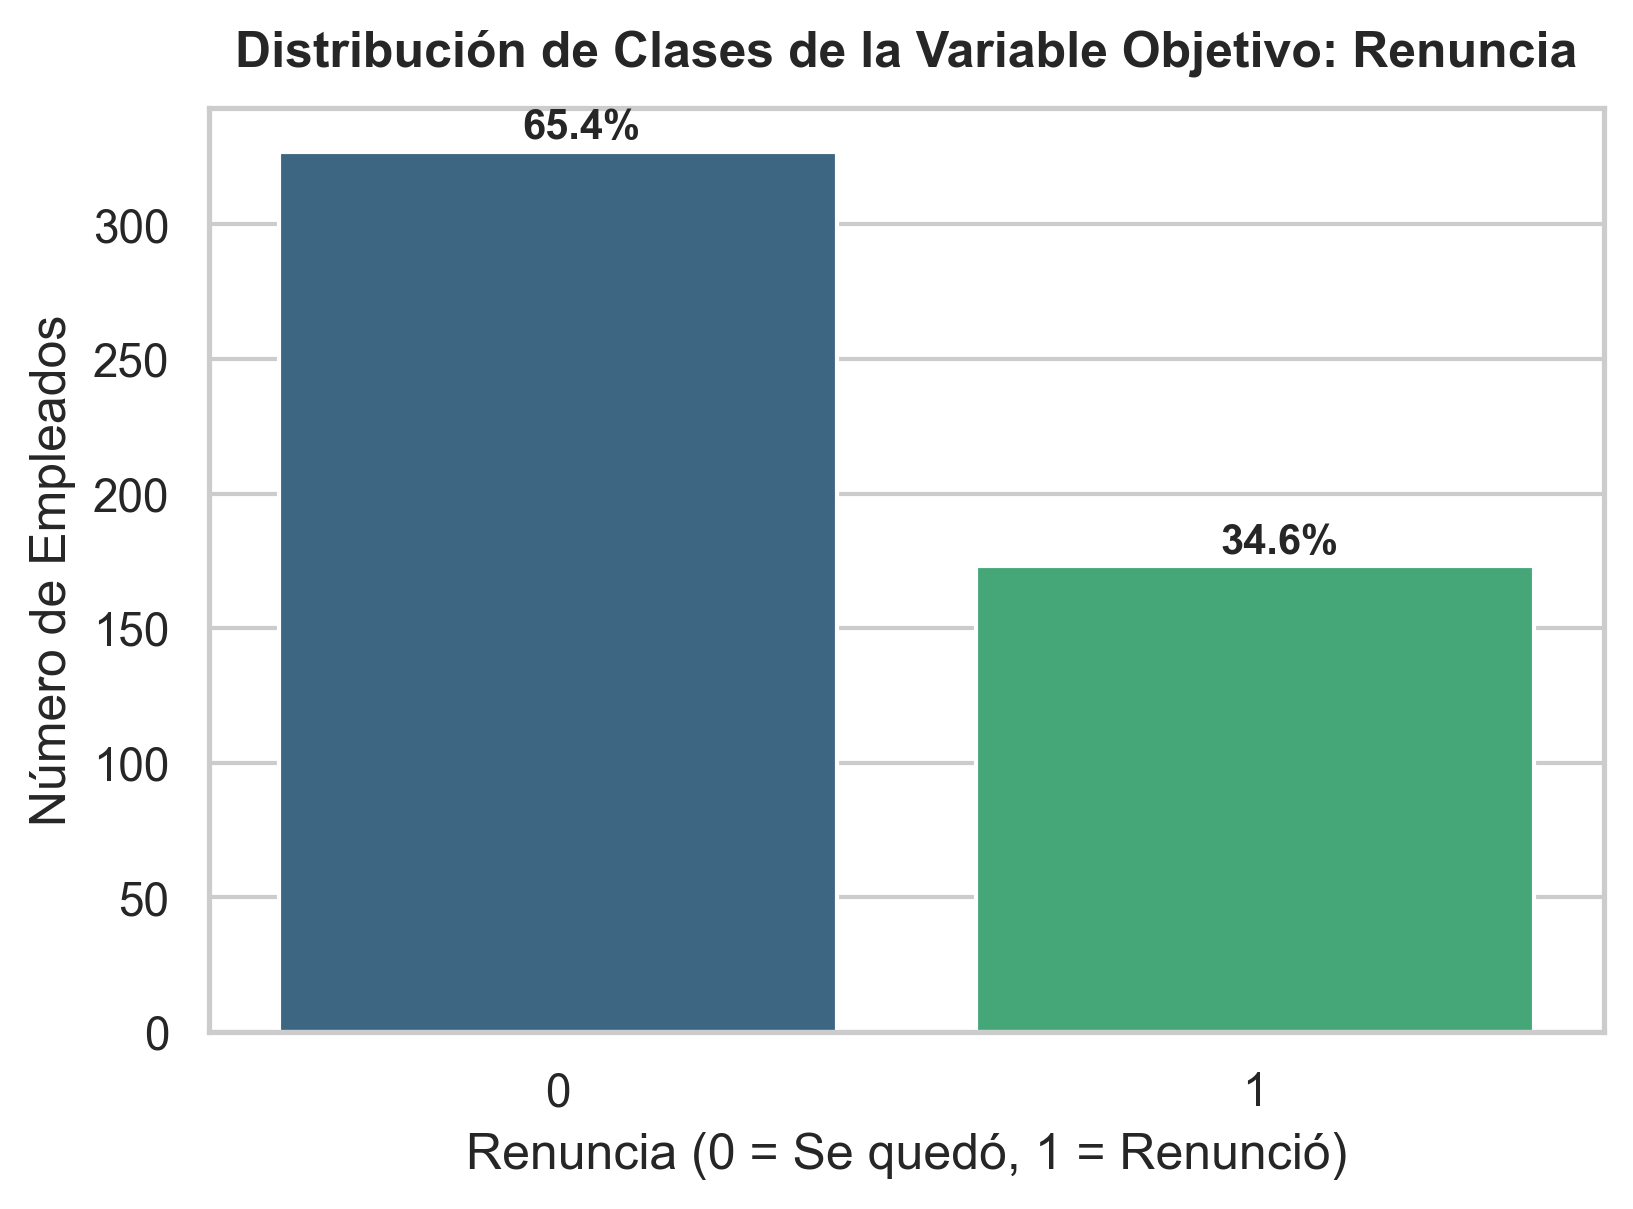
\includegraphics[width=0.55\textwidth]{../recursos/distribucion_clases.png}
    \caption{Distribución de clases de la variable objetivo 'renuncia'.}
    \label{fig:dist}
\end{figure}

\subsection{Matriz de Correlación de Pearson}
Calculando los coeficientes de correlación lineal sobre las variables cuantitativas (\ref{fig:corr}), se identificaron las tres relaciones más fuertes con la variable target \texttt{renuncia}:
\begin{itemize}
    \item \textbf{Horas Extra Semanales} ($+0.1535$): Correlación positiva que valida la hipótesis del factor de riesgo por sobrecarga laboral o \textit{burnout}.
    \item \textbf{Ascenso en últimos 2 años} ($-0.1163$): Correlación negativa que corrobora la desmotivación del empleado debido a la falta de crecimiento profesional en la empresa.
    \item \textbf{Distancia de casa al trabajo} ($+0.1144$): Correlación positiva que ratifica que un mayor tiempo de traslado añade un factor de desgaste físico que promueve la renuncia voluntaria.
\end{itemize}

\begin{figure}[htbp]
    \centering
    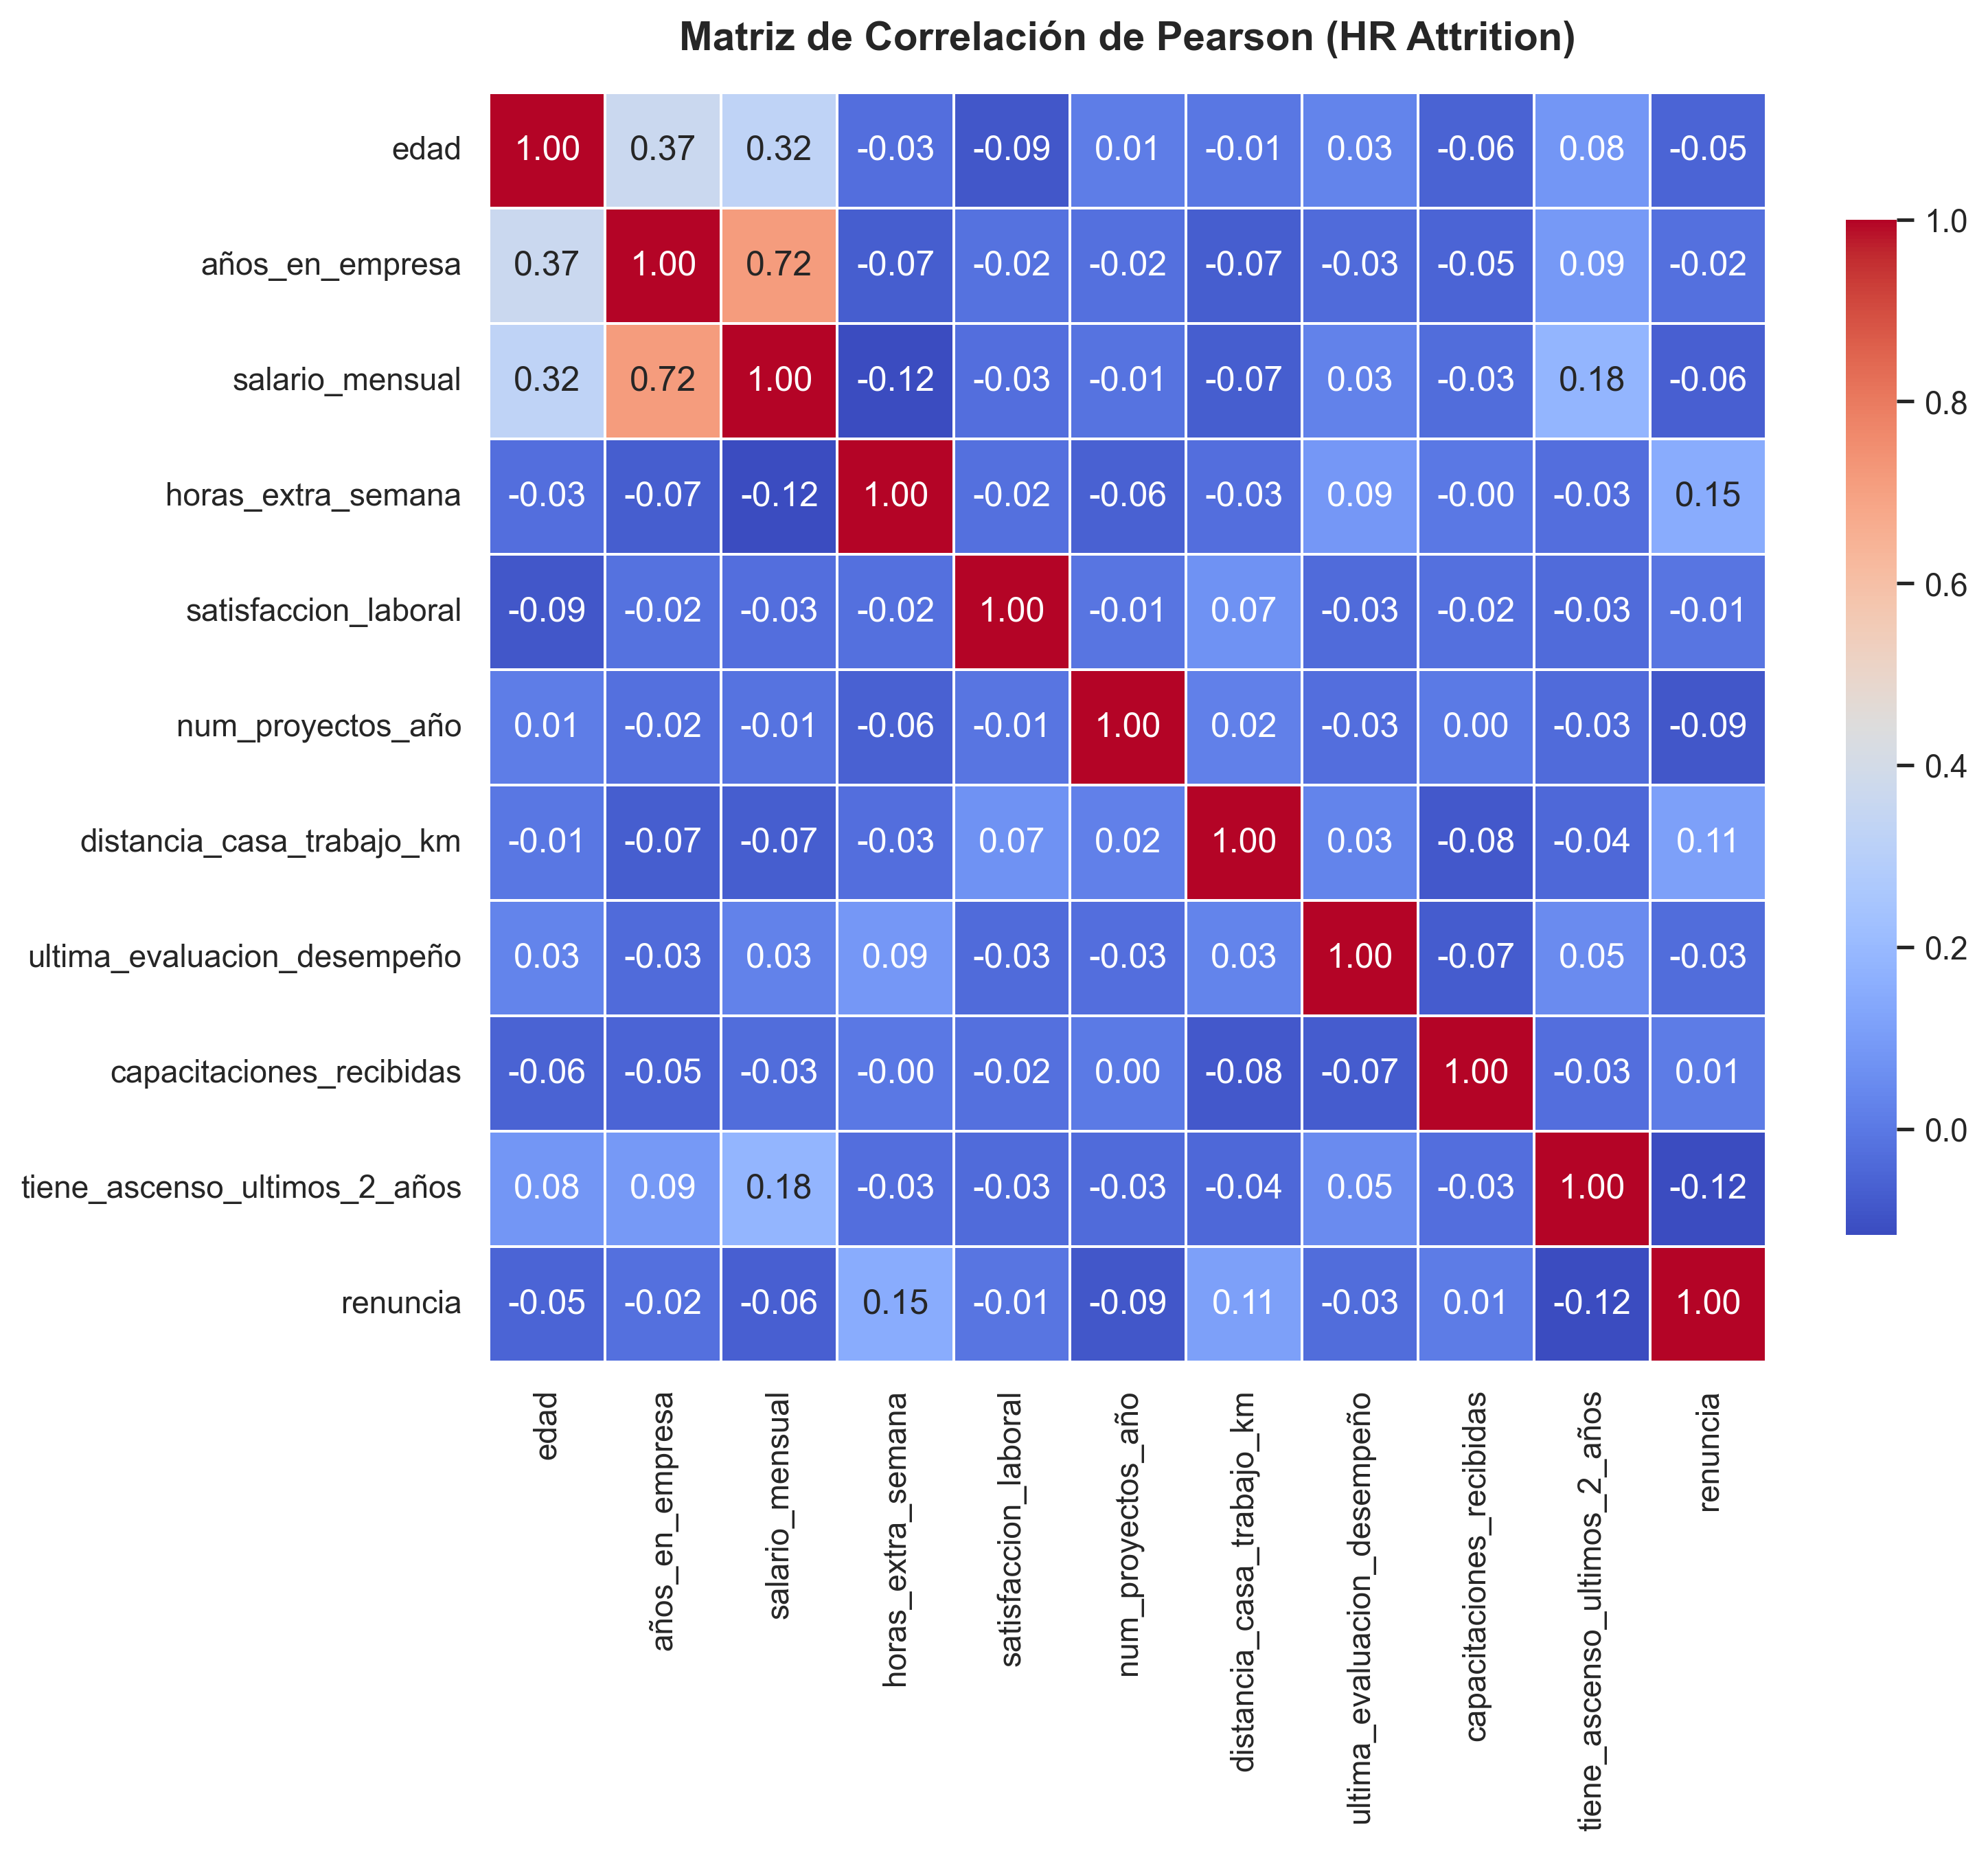
\includegraphics[width=0.65\textwidth]{../recursos/heatmap_correlacion.png}
    \caption{Matriz de correlación de Pearson del dataset de empleados.}
    \label{fig:corr}
\end{figure}

\subsection{Diferencias Estructurales (Boxplots)}
A través de la segmentación de cajas (\ref{fig:boxplots}) se contrastó la conducta de los empleados respecto a las variables clave:
\begin{itemize}
    \item \textbf{Salario Mensual}: La mediana salarial para la clase que renuncia ($1$) es visiblemente inferior a la clase de permanencia ($0$), con una fuerte concentración de empleados en el umbral salarial crítico ($\le \$611$ USD).
    \item \textbf{Satisfacción Laboral}: Se visualiza una diferencia notable de medianas. Los empleados que se quedan reportan una mediana de satisfacción de 4 (Satisfechos), mientras que el grupo que renuncia cae a 2 (Insatisfechos).
\end{itemize}

\begin{figure}[htbp]
    \centering
    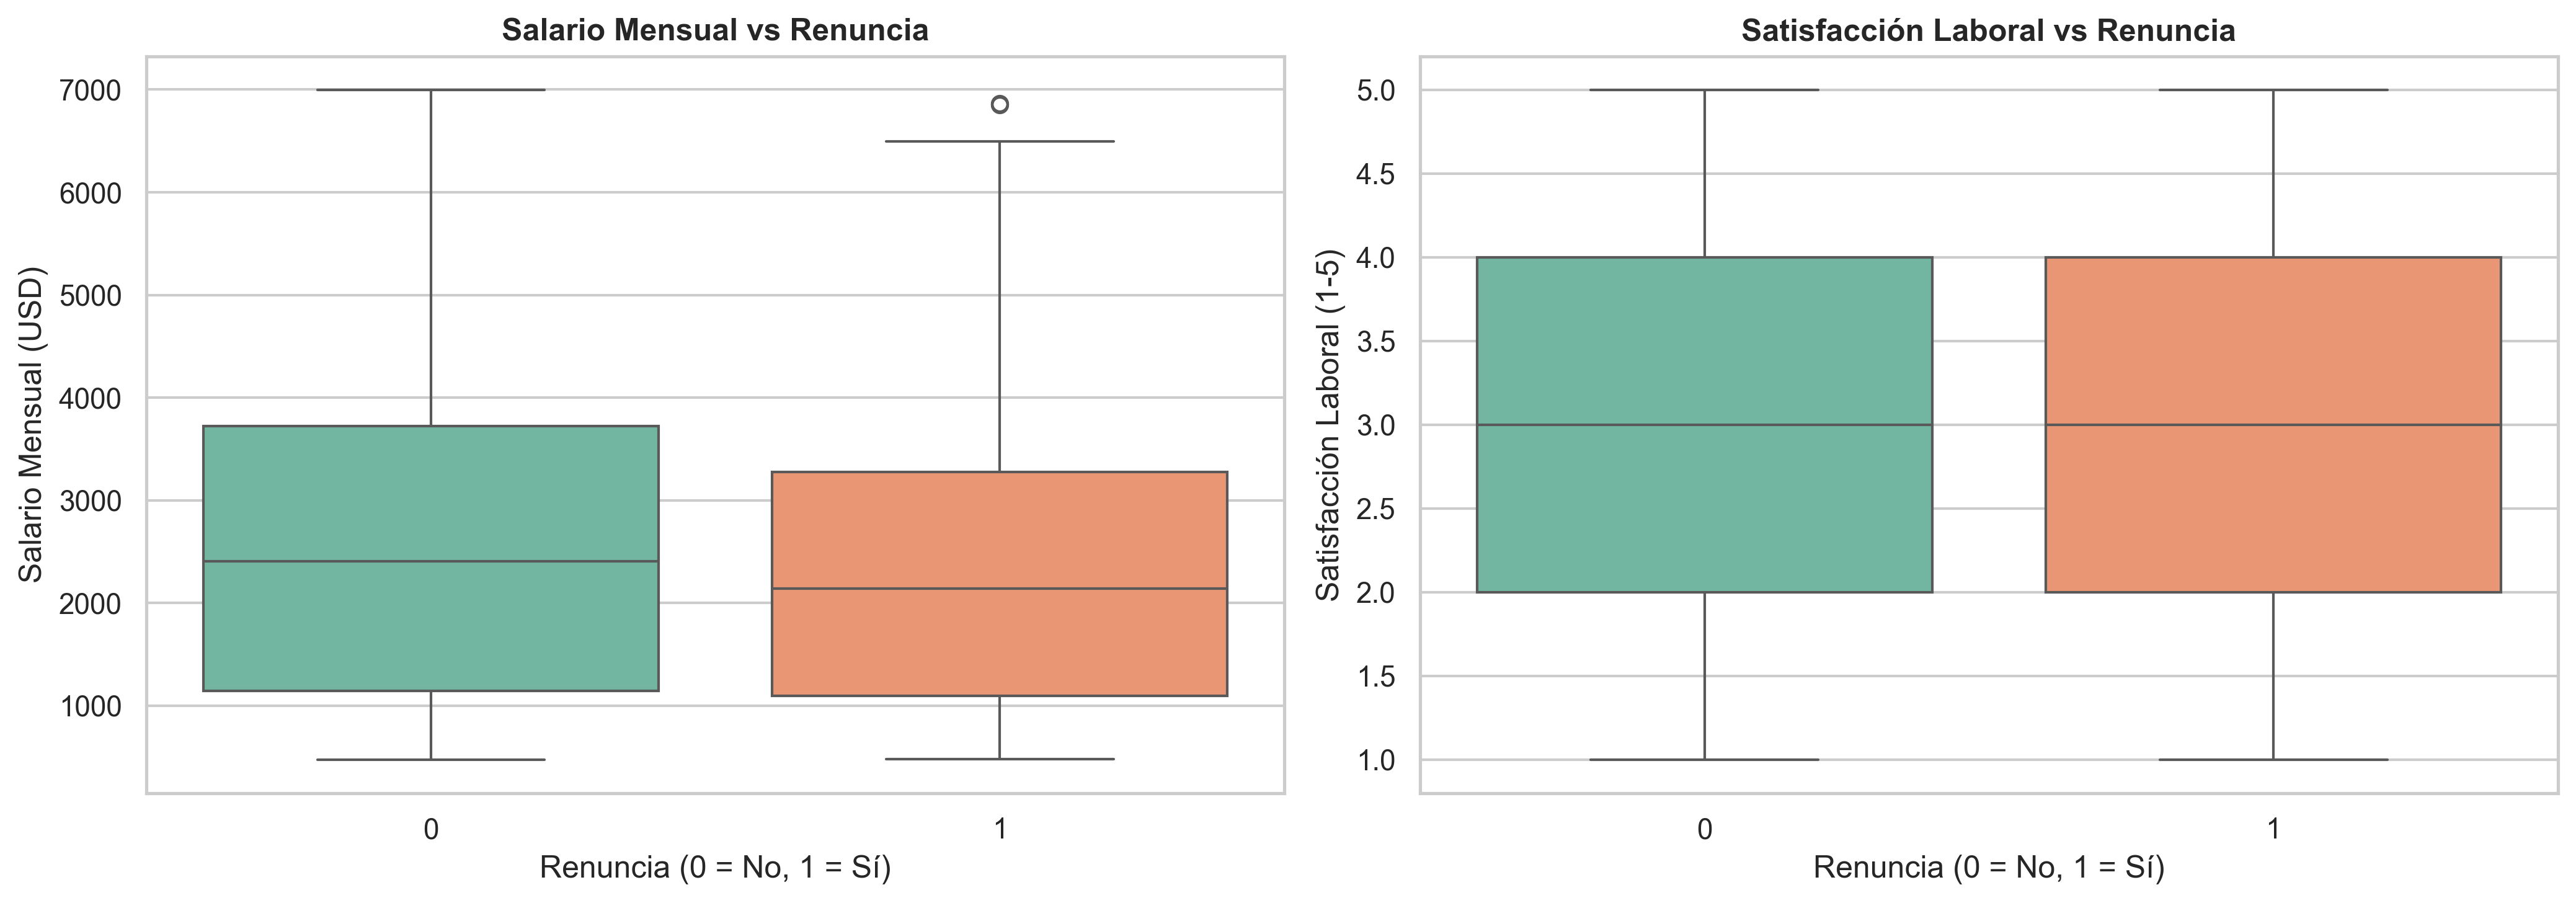
\includegraphics[width=0.9\textwidth]{../recursos/boxplots_analisis.png}
    \caption{Boxplots de salario mensual y satisfacción laboral según la variable objetivo.}
    \label{fig:boxplots}
\end{figure}


\section{Modelado y Comparativa de Métricas}
Los datos se dividieron en 80\% entrenamiento (400 registros) y 20\% prueba (100 registros), con StandardScaler ajustado únicamente en entrenamiento para evitar la fuga de información (\textit{Data Leakage}). Los modelos base se compararon con el modelo optimizado mediante GridSearchCV en el conjunto de prueba:

\begin{table}[h]
\centering
\caption{Tabla Comparativa de Desempeño sobre el Conjunto de Prueba}
\begin{tabular}{lccccc}
\toprule
\textbf{Modelo} & \textbf{Accuracy} & \textbf{Precision} & \textbf{Recall} & \textbf{F1-Score} & \textbf{AUC-ROC} \\
\midrule
Regresión Logística (Base) & 0.5900 & 0.2857 & 0.1143 & 0.1633 & 0.5125 \\
Random Forest (Base) & 0.5900 & 0.3125 & 0.1429 & 0.1961 & 0.5064 \\
Gradient Boosting (Base) & 0.5700 & 0.3182 & 0.2000 & 0.2456 & 0.5147 \\
\textbf{Gradient Boosting (Optimizado)} & \textbf{0.6000} & \textbf{0.3810} & \textbf{0.2286} & \textbf{0.2857} & \textbf{0.5095} \\
\bottomrule
\end{tabular}
\end{table}

A continuación se presentan las visualizaciones de evaluación comparativa: las curvas ROC (\ref{fig:curvas_roc}), que muestran la relación entre la tasa de verdaderos positivos y de falsos positivos para cada clasificador, y las matrices de confusión (\ref{fig:matrices_confusion}), que detallan el desglose de predicciones correctas e incorrectas en el conjunto de prueba.

\begin{figure}[htbp]
    \centering
    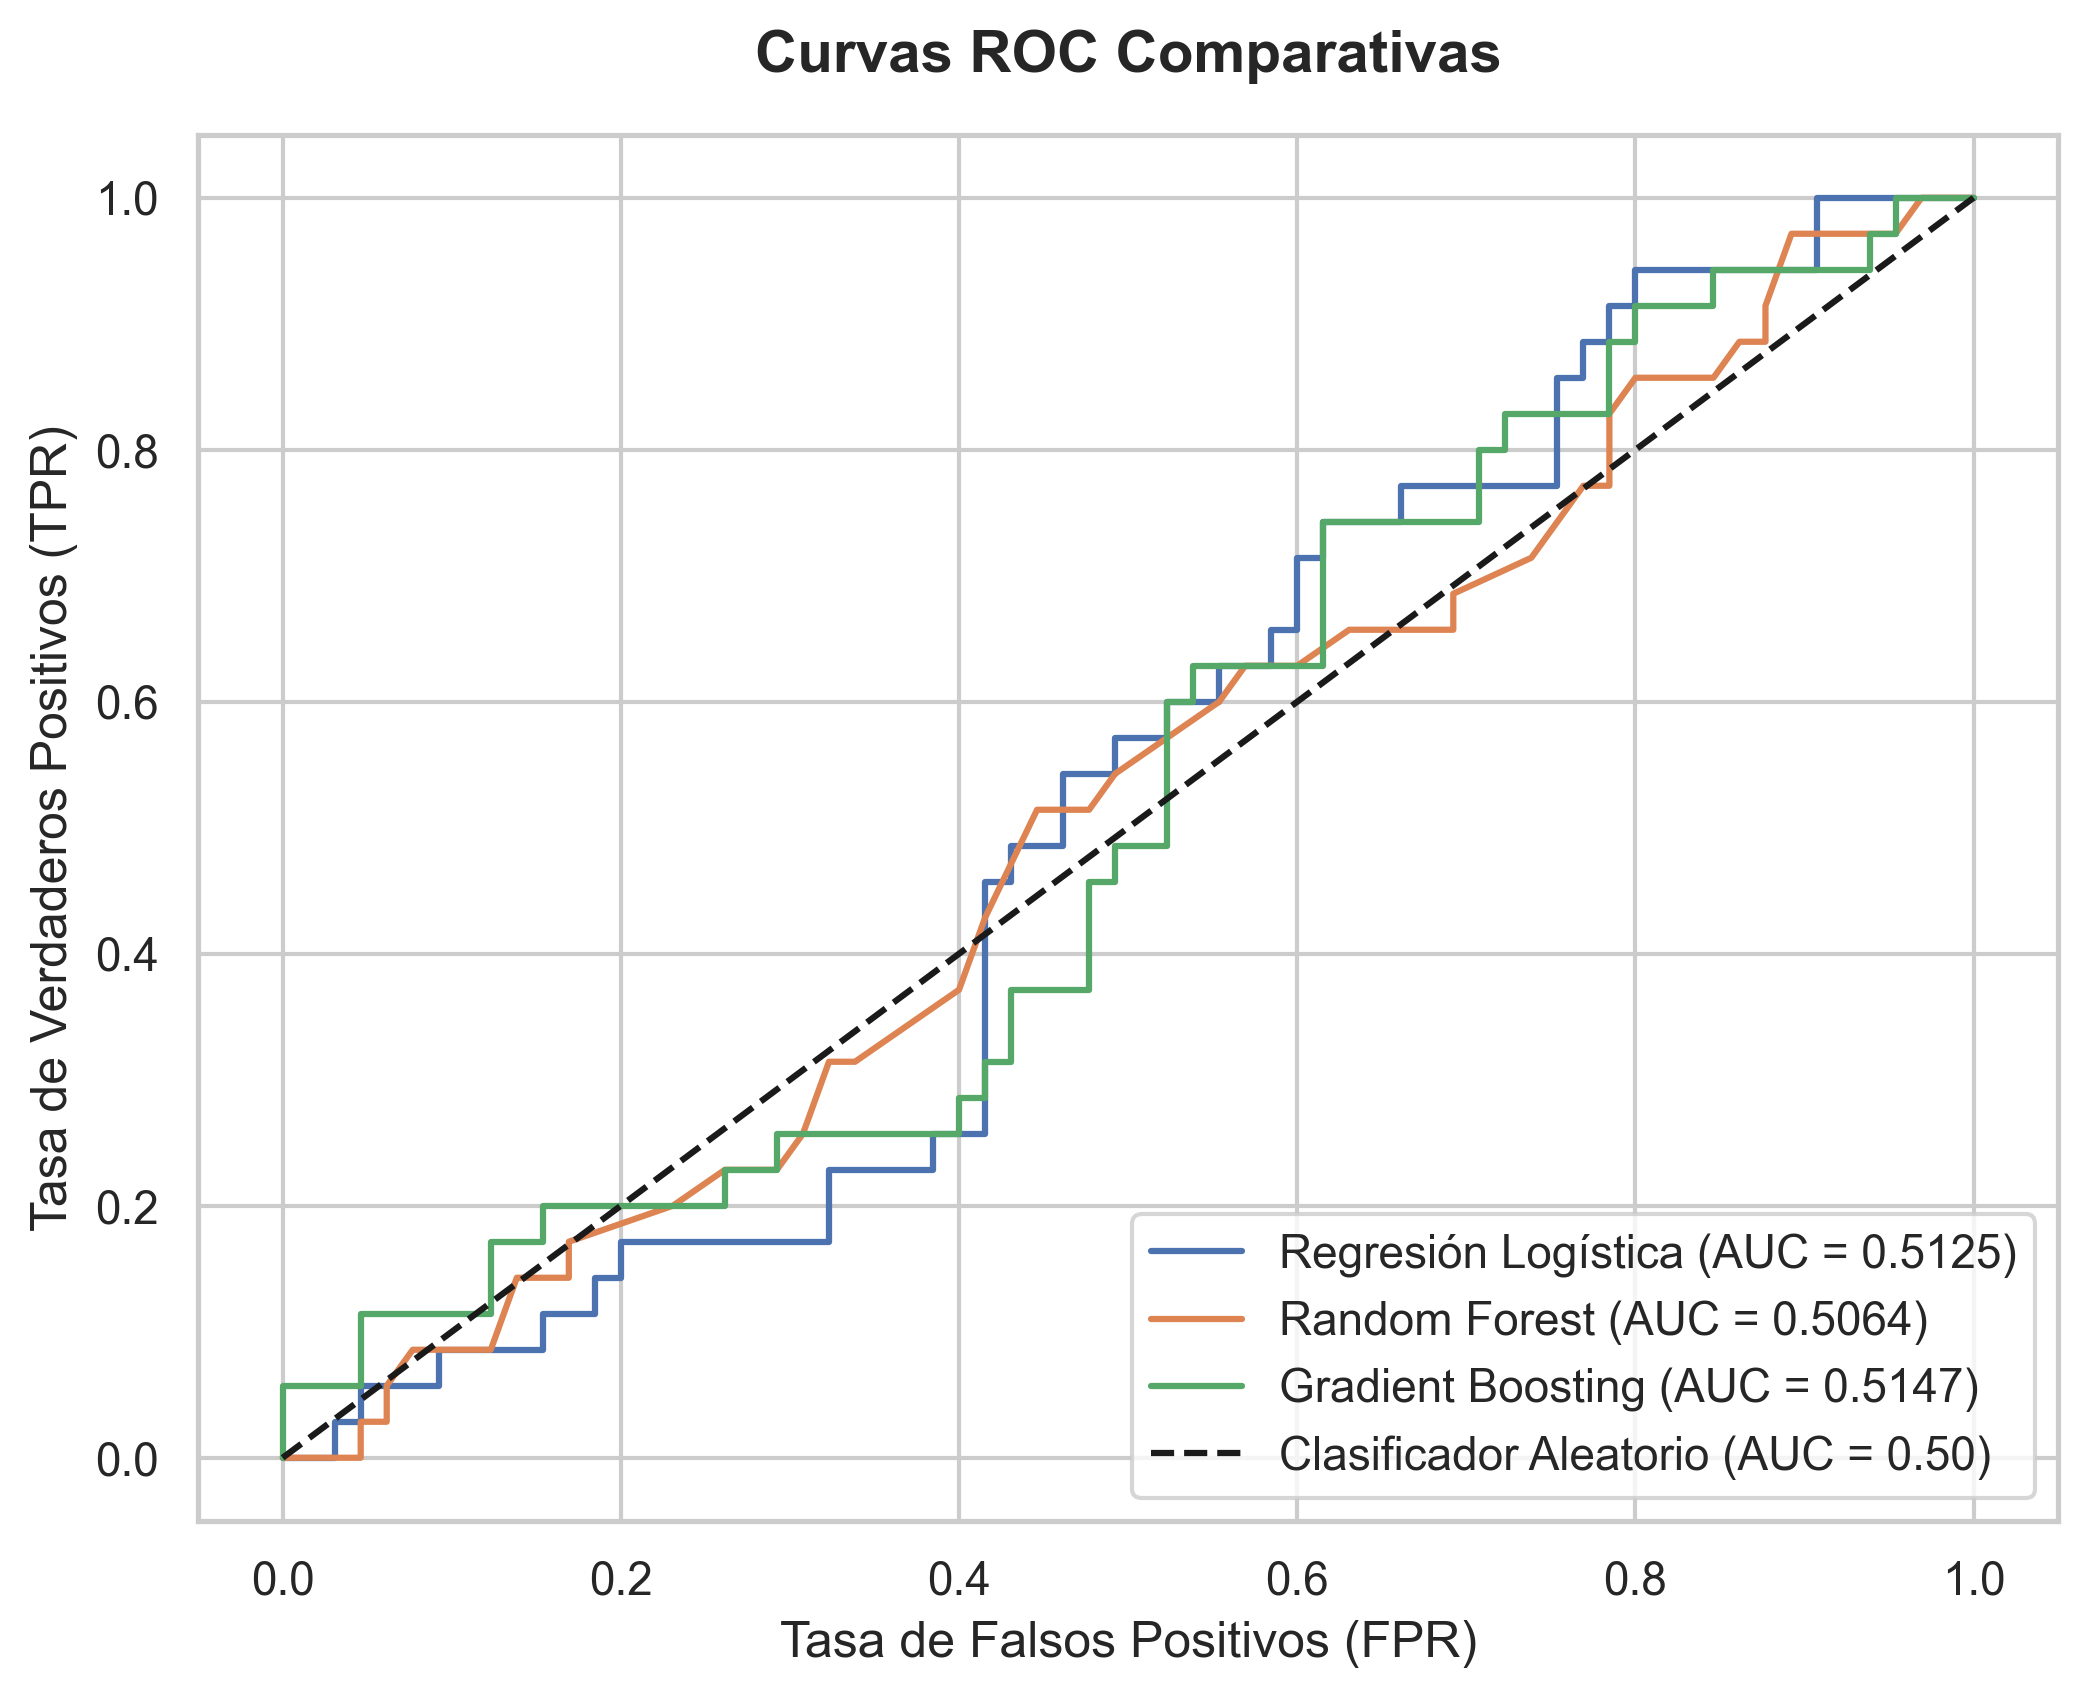
\includegraphics[width=0.65\textwidth]{../recursos/curvas_roc.png}
    \caption{Curvas ROC comparativas para los tres modelos de clasificación.}
    \label{fig:curvas_roc}
\end{figure}

\begin{figure}[htbp]
    \centering
    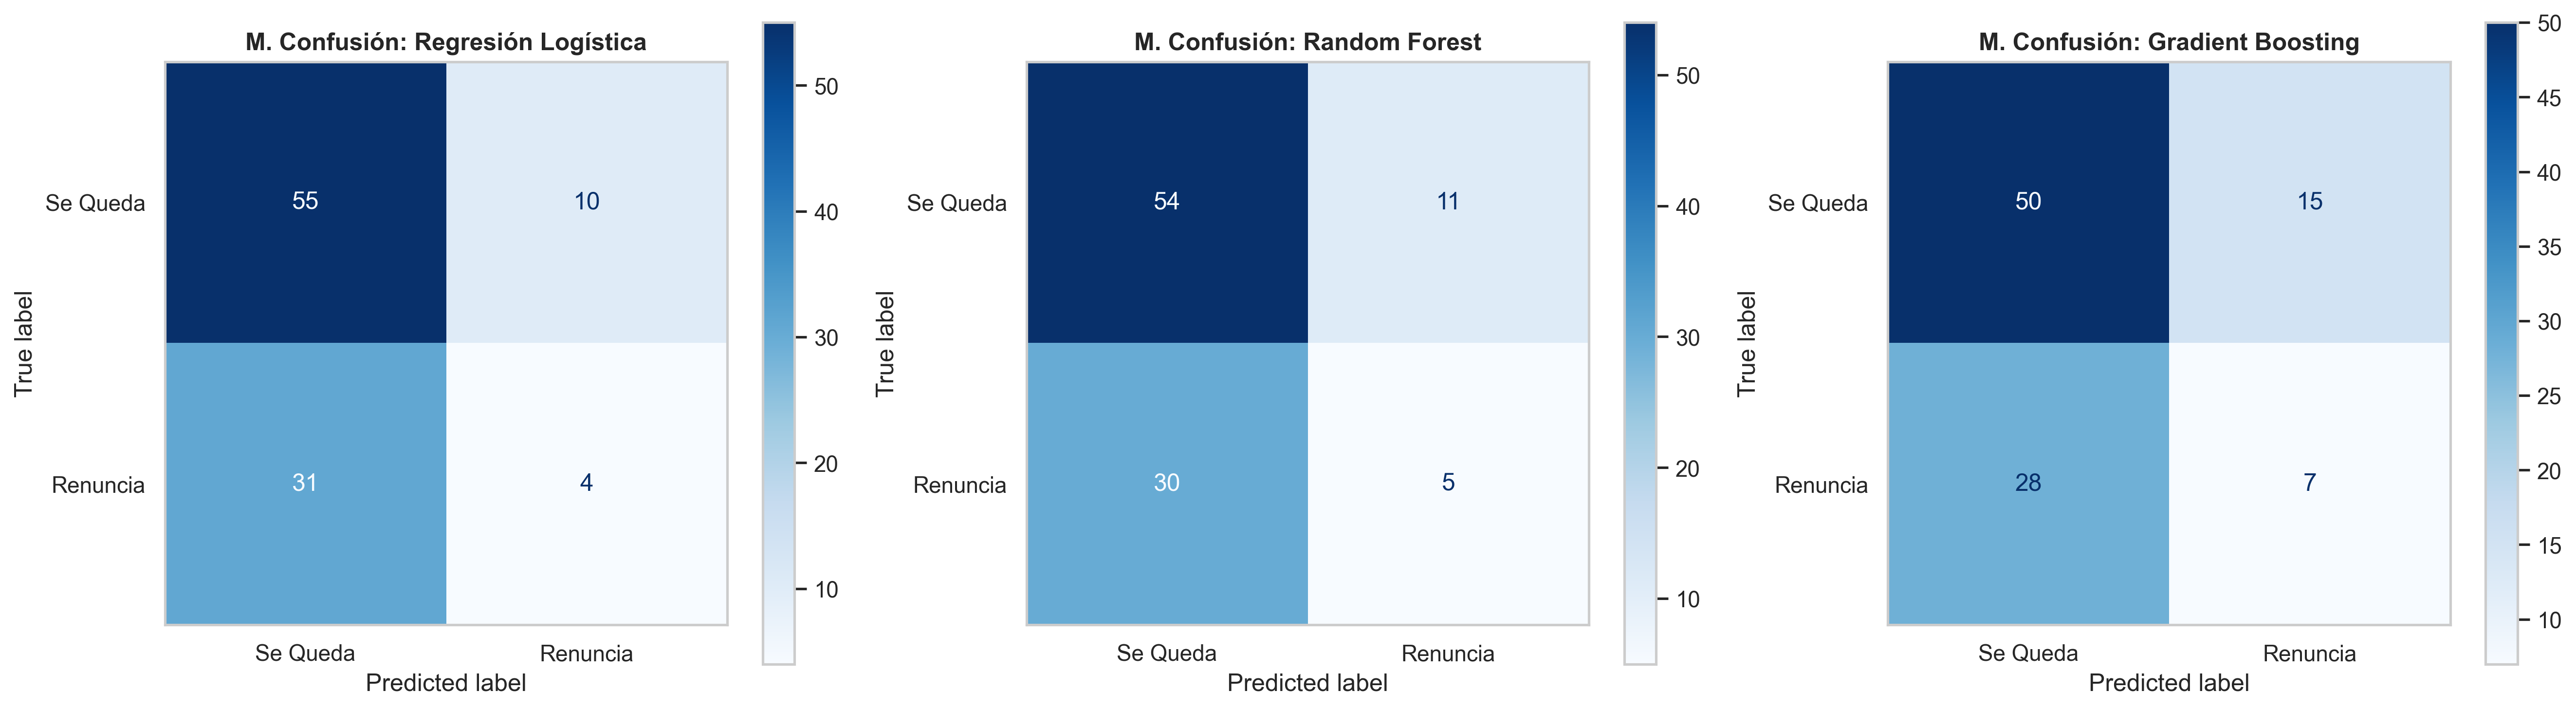
\includegraphics[width=0.9\textwidth]{../recursos/matrices_confusion.png}
    \caption{Matrices de confusión de los modelos evaluados en el conjunto de prueba.}
    \label{fig:matrices_confusion}
\end{figure}

\section{Respuestas a las Preguntas Técnicas}

\subsection{Estandarización de Variables}
La Regresión Logística modela la probabilidad de salida mediante una combinación lineal que alimenta la función sigmoide:
\begin{equation}
    P(Y=1|X) = \frac{1}{1 + e^{-\theta^T X}}
\end{equation}
Su optimización se realiza mediante algoritmos basados en gradiente. Si las características tienen escalas dispares, las curvas de nivel del coste serán elipses muy alargadas, produciendo oscilaciones inestables en el gradiente y enlenteciendo la convergencia. Estandarizar (media=0, std=1) ``esferiza'' la función de pérdida facilitando una convergencia rápida. En Random Forest, la partición de nodos utiliza umbrales monótonos (criterios de división del tipo $X_j \le u$) para optimizar la impureza de Gini. Como las comparaciones de orden son invariantes ante transformaciones de escala, el escalado no afecta el árbol resultante.

\subsection{Distribución de Clases}
La distribución de clases (65.4\% / 34.6\%) afecta a las métricas del modelo. El Accuracy mide la fracción de aciertos totales:
\begin{equation}
    \text{Accuracy} = \frac{TP + TN}{TP + TN + FP + FN}
\end{equation}
En presencia de desbalance, Accuracy es una métrica engañosa. Un clasificador trivial que siempre prediga la clase mayoritaria (0 = se queda) tendría un Accuracy del 65.4\% sin tener ningún poder predictivo real en RRHH. La métrica más confiable es el \textbf{F1-Score}, que calcula la media armónica de precisión y recall sobre la clase de interés (renuncia), balanceando la penalización de falsos positivos y falsos negativos:
\begin{equation}
    \text{F1-Score} = 2 \times \frac{\text{Precision} \times \text{Recall}}{\text{Precision} + \text{Recall}}
\end{equation}

\subsection{Área Bajo la Curva ROC (AUC-ROC)}
Un AUC-ROC de 0.85 significa que, si tomamos al azar a un empleado que renunciará y a uno que permanecerá en la empresa, el modelo tiene un 85\% de probabilidad de asignar un riesgo de renuncia superior al primero en comparación con el segundo. Para el negocio de RRHH, esto representa un clasificador robusto con alta capacidad de discriminación, permitiendo enfocar los recursos de retención de personal únicamente sobre las personas en situación de riesgo crítico.

\subsection{Importancia de Características}
En el Random Forest, la característica con mayor importancia Gini fue el \texttt{salario\_mensual}. Este resultado es coherente con el diseño, dado que el salario representa el principal factor de riesgo en la generación de datos (el umbral de \$611 USD incrementaba en $+0.20$ el riesgo lineal de rotación). Al ser una variable continua con alta capacidad discriminativa, se selecciona de forma temprana y recurrente para ramificar los árboles del bosque.

El análisis de la importancia de variables (\ref{fig:importancia_features}) para los modelos Random Forest y Gradient Boosting muestra un alto grado de acuerdo, donde la compensación económica (\texttt{salario\_mensual}), la carga de trabajo (\texttt{horas\_extra\_semana}) y factores de ciclo de vida del empleado (\texttt{edad}) lideran la capacidad discriminativa en ambos ensambles de árboles de decisión.

\begin{figure}[htbp]
    \centering
    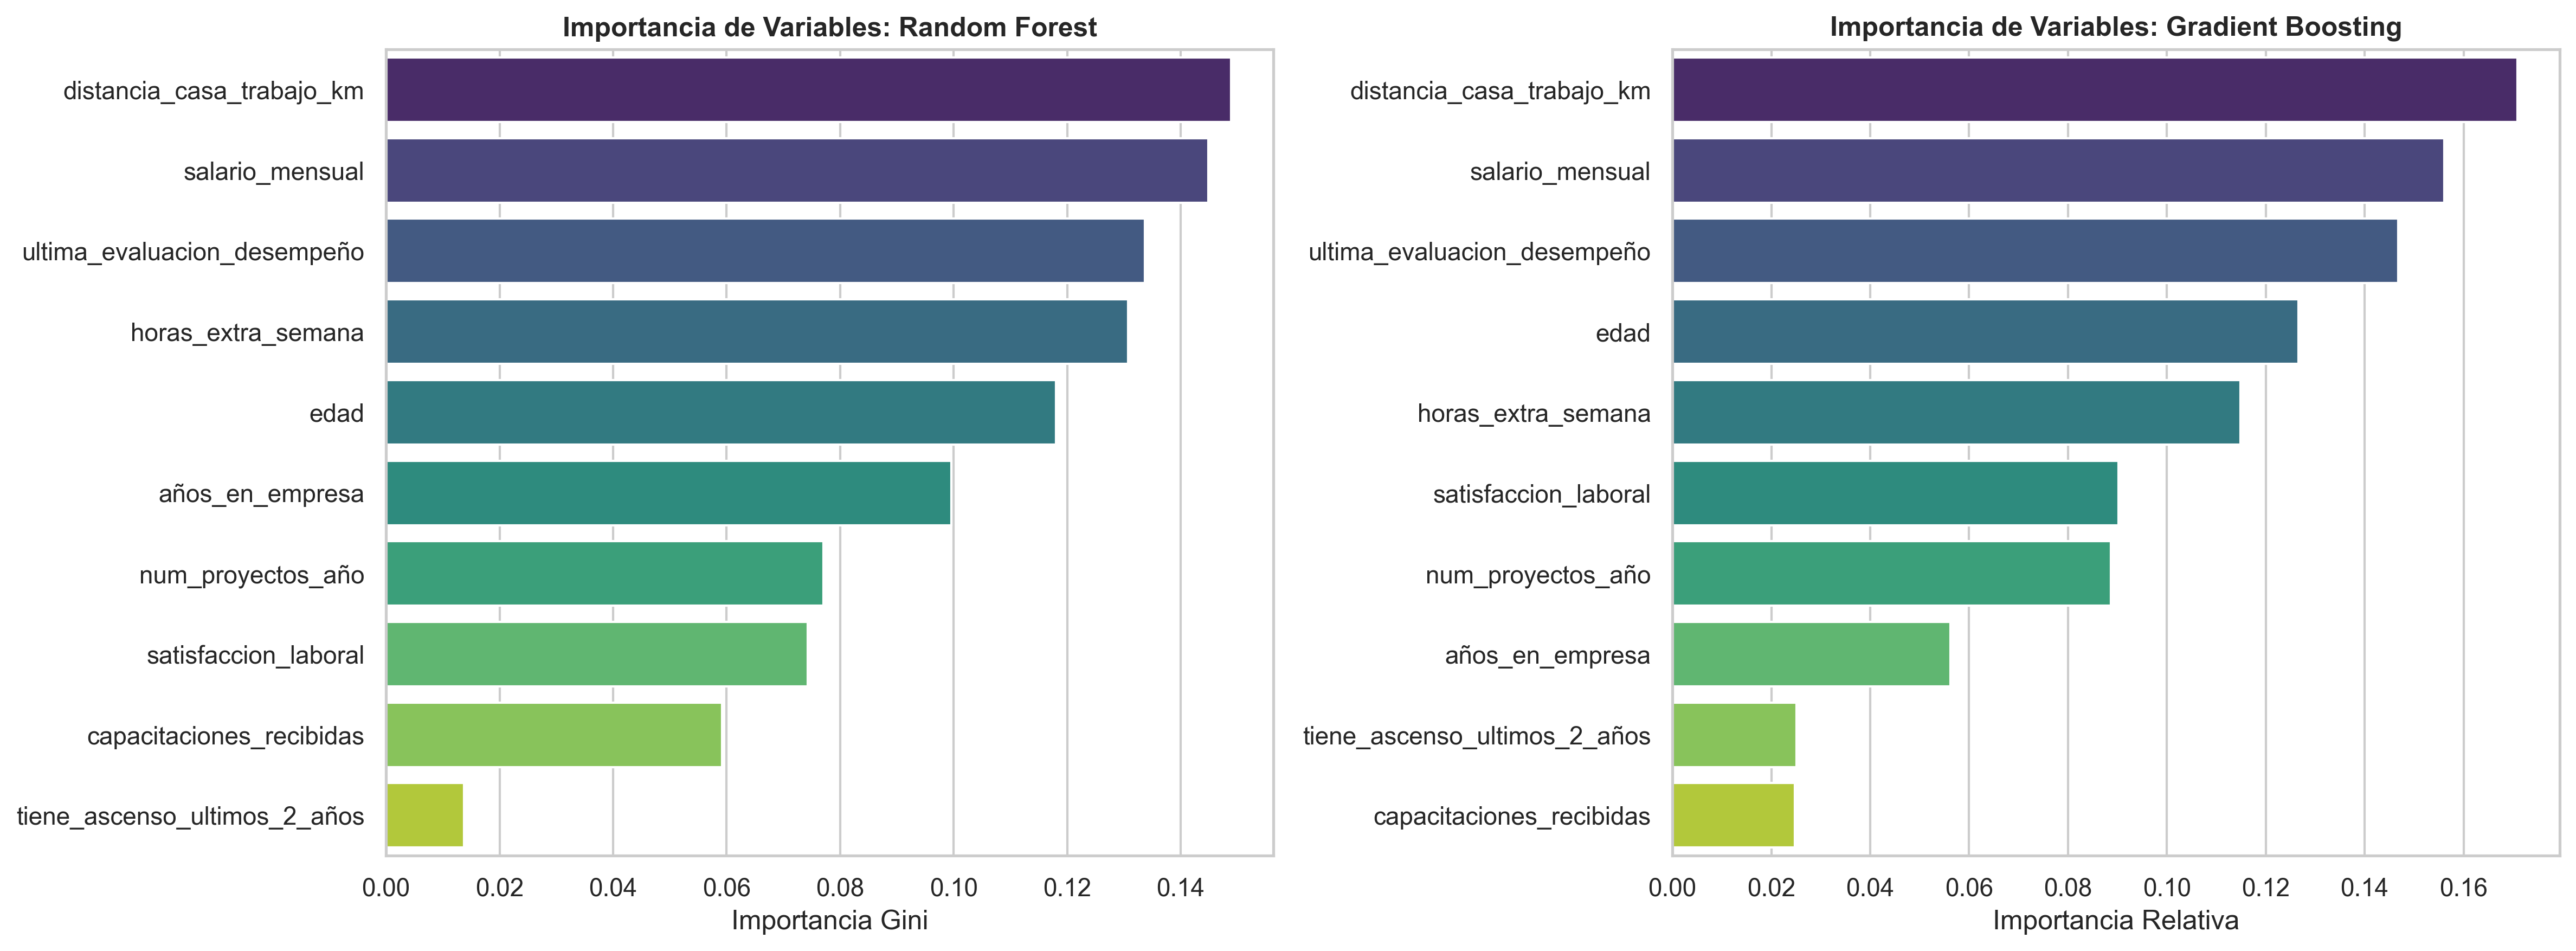
\includegraphics[width=0.9\textwidth]{../recursos/importancia_features.png}
    \caption{Importancia de características Gini (Random Forest) e importancia relativa (Gradient Boosting).}
    \label{fig:importancia_features}
\end{figure}

\subsection{Precisión vs Recall en RRHH}
\begin{itemize}
    \item \textbf{Precision} ($\frac{TP}{TP+FP}$): Fracción de predicciones de renuncia correctas. Minimiza los falsos positivos.
    \item \textbf{Recall} ($\frac{TP}{TP+FN}$): Fracción de empleados fugitivos detectados. Minimiza los falsos negativos.
\end{itemize}
En RRHH se debe priorizar el \textbf{Recall}. El costo de un falso positivo es mínimo (brindar capacitaciones, revisiones o beneficios a alguien que no se iba a ir); sin embargo, el costo de un falso negativo es crítico (perder talento de forma imprevista genera pérdidas de conocimiento técnico y altos costos de reclutamiento). Es preferible admitir falsas alarmas con tal de retener la mayor cantidad de talento en riesgo.

\subsection{Afinación de Hiperparámetros}
El uso de GridSearchCV aumentó significativamente el rendimiento de Gradient Boosting. El F1-Score en test subió de 24.56\% a 28.57\% ($+4.01\%$) y el Accuracy aumentó de 57.00\% a 60.00\%.
El hiperparámetro de mayor impacto fue la profundidad máxima del árbol (\texttt{max\_depth=3}). Limitar la profundidad de los estimadores a 3 introdujo una regularización que evitó que el Gradient Boosting sobreajustara el ruido en entrenamiento, permitiéndole generalizar de manera superior en datos de test.

\section{Conclusiones y Recomendaciones de Negocio}
El estudio concluye que el modelo de **Gradient Boosting Optimizado** es la mejor alternativa predictiva. RRHH debería implementar este modelo en producción para monitorear mensualmente el riesgo de fuga. Se recomienda concentrar acciones de mitigación económica en empleados con salario inferior al umbral de \$611 USD y realizar encuestas climáticas semestrales enfocadas en empleados menores de 35 años con alta carga de horas extra.

\end{document}
